%%%%%%%%%%%%%%%%%%%%%%%%%%%%%%%%%%%%%%%%%%%%%%%%%%%%%%%%%%%%%%%%%%%%%%
%     File: ExtendedAbstract_imple.tex                               %
%     Tex Master: ExtendedAbstract.tex                               %
%%%%%%%%%%%%%%%%%%%%%%%%%%%%%%%%%%%%%%%%%%%%%%%%%%%%%%%%%%%%%%%%%%%%%%

\section{Aerial-D Dataset Construction}
\label{sec:approach}

This section details our comprehensive approach to constructing Aerial-D, the largest referring segmentation dataset for aerial imagery. Our methodology combines automated rule-based expression generation with large language model enhancement to achieve both scale and linguistic diversity. We begin by establishing our source datasets, then describe our rule-based pipeline for generating referring expressions from existing annotations, followed by our novel knowledge distillation approach for cost-effective LLM enhancement, and conclude with comprehensive dataset statistics demonstrating the scope and characteristics of the final resource.

\subsection{Source Datasets}

The Aerial-D dataset is constructed from two complementary aerial benchmarks with different annotation styles: iSAID (instance segmentation) and LoveDA (semantic segmentation).

We start by putting both sources into the same format so that a single model can learn from them side by side: square patches at 480×480. This size keeps small iSAID objects large enough to describe and segment, while fitting the input expectations of common vision encoders used in our model (e.g., CLIP/SigLIP image towers and SAM backbones\cite{clip,siglip,sam}).

From there, preparation is straightforward. For iSAID’s very large images, we use an overlapping sliding window and keep the patches that contain valid instances. For LoveDA, we resize to the same patch size and derive instance targets for the classes of interest—buildings and water—using connected-component analysis on the semantic masks. We also retain the full semantic labels per patch. Buildings and water are amenable to instance-level treatment; while water is a land-cover class, in LoveDA it predominantly appears as well-defined lakes and some rivers, which people naturally refer to as discrete entities or sets. Other land-cover classes (e.g., farmland or forest) behave as continuous surfaces, so splitting them into arbitrary components would create unnatural targets for referring expressions. We therefore keep those land-cover classes at the category level with encompassing descriptions, while promoting buildings and water to instance targets. The result is a unified per-patch representation with instance targets and complete category labels, which we then use for rule-guided expression generation.

\subsection{Rule-Based Expression Generation}

The core challenge is figuring out how to describe these target objects using only what we know from their bounding boxes, masks, and categories. We utilize the bounding box coordinates to understand where each object sits within the image patch. As shown in Figure \ref{fig:rule_example}, we divide each patch into a three-by-three grid marked with dotted lines, so we can say an object is "in the top right" or "in the center". When we have multiple objects of the same type, we also check if any are in extreme positions like the topmost or leftmost instance of that category.

Since we also have the pixel masks for each object, we can analyze their colors by looking at HSV values to distinguish between light and dark objects, and various chromatic colors. However, we avoid using color descriptions for buildings and water since these typically show mixed colors that aren't useful for identification.

We also create relationships between nearby objects by calculating angles between their positions, allowing us to generate expressions like "the ship to the left of the harbor" or "the vehicle above the building". The system uses eight directional relationships: above, below, to the left of, to the right of, and the four diagonal directions.

All these rules combine to generate various referring expressions for each object, as demonstrated in Figure \ref{fig:rule_example} where a single plane generates multiple possible descriptions including "the plane in the top right", "the light plane in the top right", and versions with relational descriptions. However, a significant challenge emerges when multiple objects end up with identical characteristics and generate the exact same expressions, creating ambiguous references where one phrase could describe multiple different objects. We solve this fundamental problem by taking the set of all expressions for all objects and targets in each image, matching them against each other to find duplicates, and when we find expressions that are identical, we cancel both expressions out and discard them as ambiguous. This ensures every remaining phrase points to exactly one target.

\begin{figure*}[t]
\centering
\begin{minipage}{0.5\textwidth}
\centering
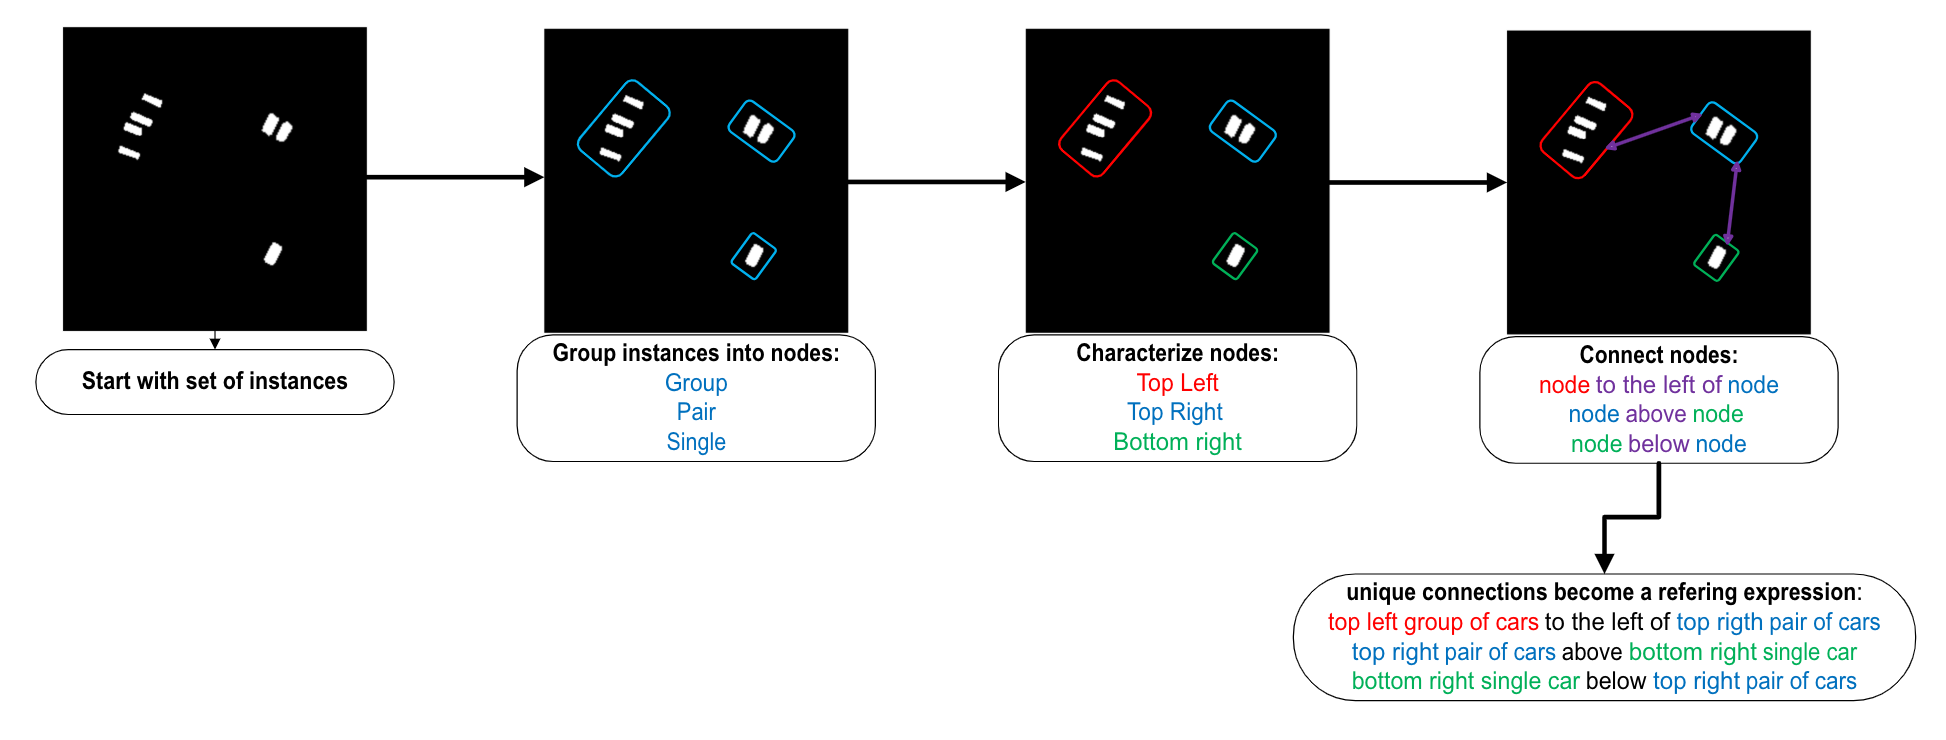
\includegraphics[width=0.65\textwidth]{./images/rule_based_generation.png}
\end{minipage}%
\begin{minipage}{0.5\textwidth}
\centering
\hspace{-1cm}
\raisebox{-0.3\height}{%
\resizebox{\textwidth}{!}{%
\footnotesize
\begin{tabular}{@{}ll@{}}
\toprule
\textbf{Rule Type} & \textbf{Example Instance} \\
\midrule
Category & "plane" \\
Grid Position & "in the top right" \\
Extreme Position & None \\
Color Classification & "light" \\
Directional Relations & "to the bottom right of a plane" \\
& "to the top right of a plane" \\
\midrule
\multicolumn{2}{l}{\textbf{Final Expressions}} \\
\multicolumn{2}{l}{"the plane in the top right"} \\
\multicolumn{2}{l}{"the light plane in the top right"} \\
\multicolumn{2}{l}{"the plane in the top right to the bottom right of a plane"} \\
\multicolumn{2}{l}{"the light plane in the top right to the bottom right of a plane"} \\
\multicolumn{2}{l}{"the plane in the top right to the top right of a plane"} \\
\multicolumn{2}{l}{"the light plane in the top right to the top right of a plane"} \\
\bottomrule
\end{tabular}%
}%
}
\end{minipage}
\caption{Example of rule generation for a single instance. The highlighted plane in the top right section demonstrates how the system assigns spatial, visual, and relational rules that will later be combined into referring expressions.}
\label{fig:rule_example}
\end{figure*}


\subsection{LLM Expression Generation}
\label{subsec:llm_expression_generation}
While rule-based expression generation provides a solid foundation for referring expression data, these expressions suffer from significant limitations in language variation and visual detail coverage. The rule-based approach produces linguistically constrained expressions with limited wording variations and lacks the ability to reference contextual elements beyond predefined source dataset categories.

To address these limitations, we employ a multimodal Large Language Model (LLM) to enhance our dataset by providing both images and expressions as input, enabling the model to rewrite and improve the original referring expressions. We target enhancement from two approaches, as shown in Figure \ref{fig:llm_enhancement_example}. The first approach focuses on linguistic variation, creating natural language alternatives for each rule-based expression without heavy reliance on visual information. The second approach uses visual information, where the model examines surrounding features in the image around the target object. We provide bounding box annotations to help the model focus on the correct target region, as demonstrated in Figure \ref{fig:llm_enhancement_example} with the group of large vehicles.

This dual approach transforms basic expressions like "the group of 4 large vehicles in the top center" into linguistically diverse alternatives such as "the cluster of four big vehicles near the upper middle" and visually detailed descriptions like "the four large vehicles lined up side by side just below the pale paved strip at the very top middle", where the model identifies and references contextual elements not captured in the original datasets, such as the "pale paved strip" and the "grassy area".

However, the full dataset contains approximately 300,000 captured targets including both objects and groups. To generate expressions, we process each target individually, meaning we would need 300,000 separate LLM requests. Using production-grade LLMs at this scale—for example, OpenAI’s o3 model\cite{o3} with strong visual capabilities—would cost thousands of dollars; Table \ref{tab:cost_comparison} reports the exact breakdown, making direct application prohibitively expensive for research-scale dataset construction.

To address this scalability challenge, we employ a knowledge distillation approach, as illustrated in Figure \ref{fig:llm_distillation}. We utilize OpenAI’s o3 model\cite{o3} and compare it against a much more lightweight open‑weights model, Gemma3\cite{gemma3}. We obtain 500 high‑quality outputs from o3 on a representative random subset of targets from the initial dataset. These outputs serve as training data for supervised fine‑tuning using the parameter‑efficient QLoRA method\cite{qlora} on Gemma3‑12B.

The custom‑tailored fine‑tuned Gemma3 model can then process all 300,000 targets using a single GPU, resulting in a much cheaper and more efficient method. Notably, the distilled model’s output quality approaches o3’s once fine‑tuned; qualitative comparisons in Figure \ref{fig:distillation_comparison} show closely matched enhancements with markedly reduced hallucinations relative to the base Gemma3 model.

\begin{figure*}[t]
\centering
\begin{minipage}{0.5\textwidth}
\centering
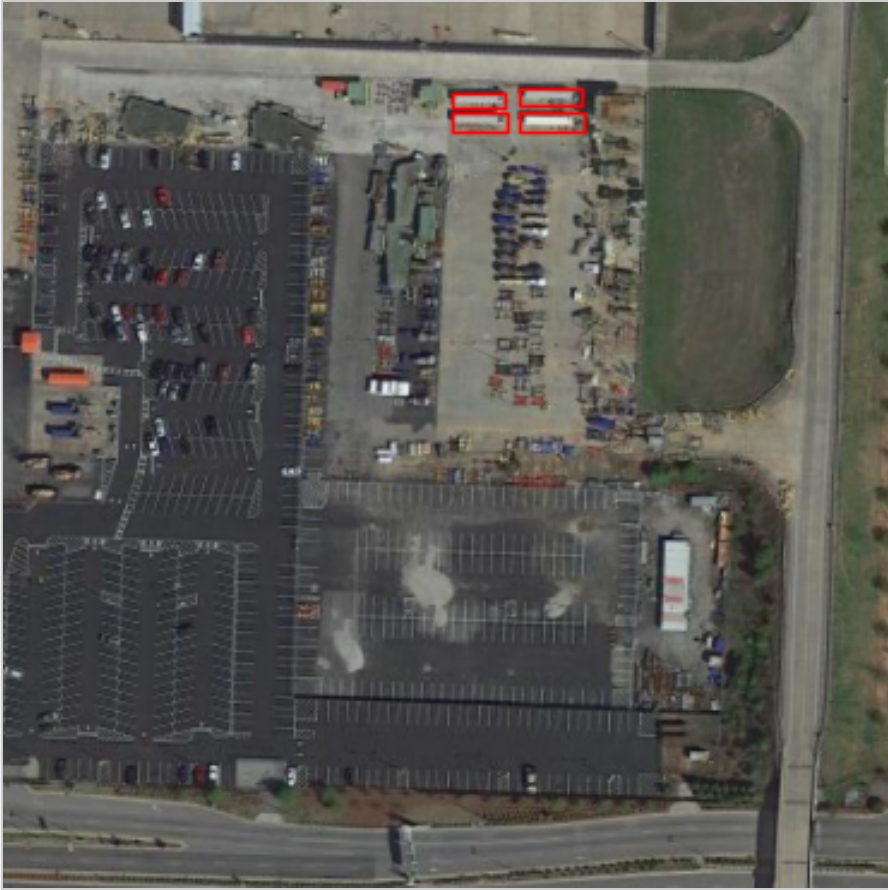
\includegraphics[width=0.65\textwidth]{./images/example_group.png}
\end{minipage}%
\begin{minipage}{0.5\textwidth}
\centering
\hspace{-1cm}
\raisebox{-0.3\height}{%
\footnotesize
\begin{tabular}{@{}p{2cm}p{5cm}@{}}
\toprule
\textbf{Expression Type} & \textbf{Example} \\
\midrule
Original & the group of 4 large vehicles in the top center \\
\midrule
Enhanced & the cluster of four big vehicles near the upper middle \\
\midrule
Unique & the four large vehicles lined up side by side just below the pale paved strip at the very top middle \\
\midrule
Unique & the set of four big vehicles parked in a single row in the upper center beside the grassy area to the right \\
\bottomrule
\end{tabular}%
}
\end{minipage}
\caption{Example of LLM enhancement process showing original aerial image with group of four large vehicles (left) and corresponding expression enhancements (right).}
\label{fig:llm_enhancement_example}
\end{figure*}


% (moved later to improve float ordering and reduce gaps)

\subsection{Historic Image Filter Augmentation}
\label{subsec:historic_filters}

In order to improve robustness to archival image conditions, we augment training with three parametric transformations that reproduce characteristic degradations of historical aerial photographs: monochrome capture, contrast roll‑off with film grain, and sepia toning with scan noise (see Figure~\ref{fig:historic_filters}). 

Let $I_{orig}(x)\in[0,255]^3$ denote the RGB image at pixel $x$, and let $\operatorname{clip}(\cdot)$ clamp values to $[0,255]$.

We simulate grayscale capture by converting to luminance, as in \eqnref{eq:gray}:
\begin{equation}
I_{\text{bw}}(x) = 0.299\,R(x) + 0.587\,G(x) + 0.114\,B(x).
\label{eq:gray}
\end{equation}

To emulate film response and grain, we first apply a mild gamma adjustment (\eqnref{eq:gamma}), then a linear contrast change around the mean (\eqnref{eq:contrast}), followed by additive Gaussian noise (\eqnref{eq:grain}):
\begin{equation}
I_{\gamma}(x) = 255\,\big(I_{\text{bw}}(x)/255\big)^{\gamma}.
\label{eq:gamma}
\end{equation}
\begin{equation}
I_{c}(x) = \big(I_{\gamma}(x) - \mu\big)\,c + \mu.
\label{eq:contrast}
\end{equation}
\begin{equation}
I_{\text{grain}}(x) = \operatorname{clip}\big(I_{c}(x) + \eta(x)\big),\quad \eta(x)\sim\mathcal{N}(0,\sigma^2).
\label{eq:grain}
\end{equation}
We use $\gamma=1.1$, $c=0.85$, and $\sigma=0.1\times 255$ to produce mild contrast loss and film grain.

Finally, we apply a fixed sepia transform (\eqnref{eq:sepia}) followed by uniform sensor/scan noise (\eqnref{eq:sepia_noise}):
\begin{equation}
\begin{bmatrix} S_R(x) \\ S_G(x) \\ S_B(x) \end{bmatrix}
= \operatorname{clip}\left(
\begin{bmatrix}
0.272 & 0.534 & 0.131 \\
0.349 & 0.686 & 0.168 \\
0.393 & 0.769 & 0.189
\end{bmatrix}
\begin{bmatrix} R(x) \\ G(x) \\ B(x) \end{bmatrix}
\right).
\label{eq:sepia}
\end{equation}
\begin{equation}
I_{\text{sepia}}(x) = \operatorname{clip}\big(\mathbf{S}(x) + \xi(x)\big),\quad \xi(x)\sim\mathcal{U}(0,50).
\label{eq:sepia_noise}
\end{equation}

These effects mimic tonal range reduction and graininess typical of mid‑century aerial photography while preserving the spatial structure that segmentation relies on. Figure~\ref{fig:historic_filters} illustrates the visual impact of each transformation.

\begin{figure*}[t]
\centering
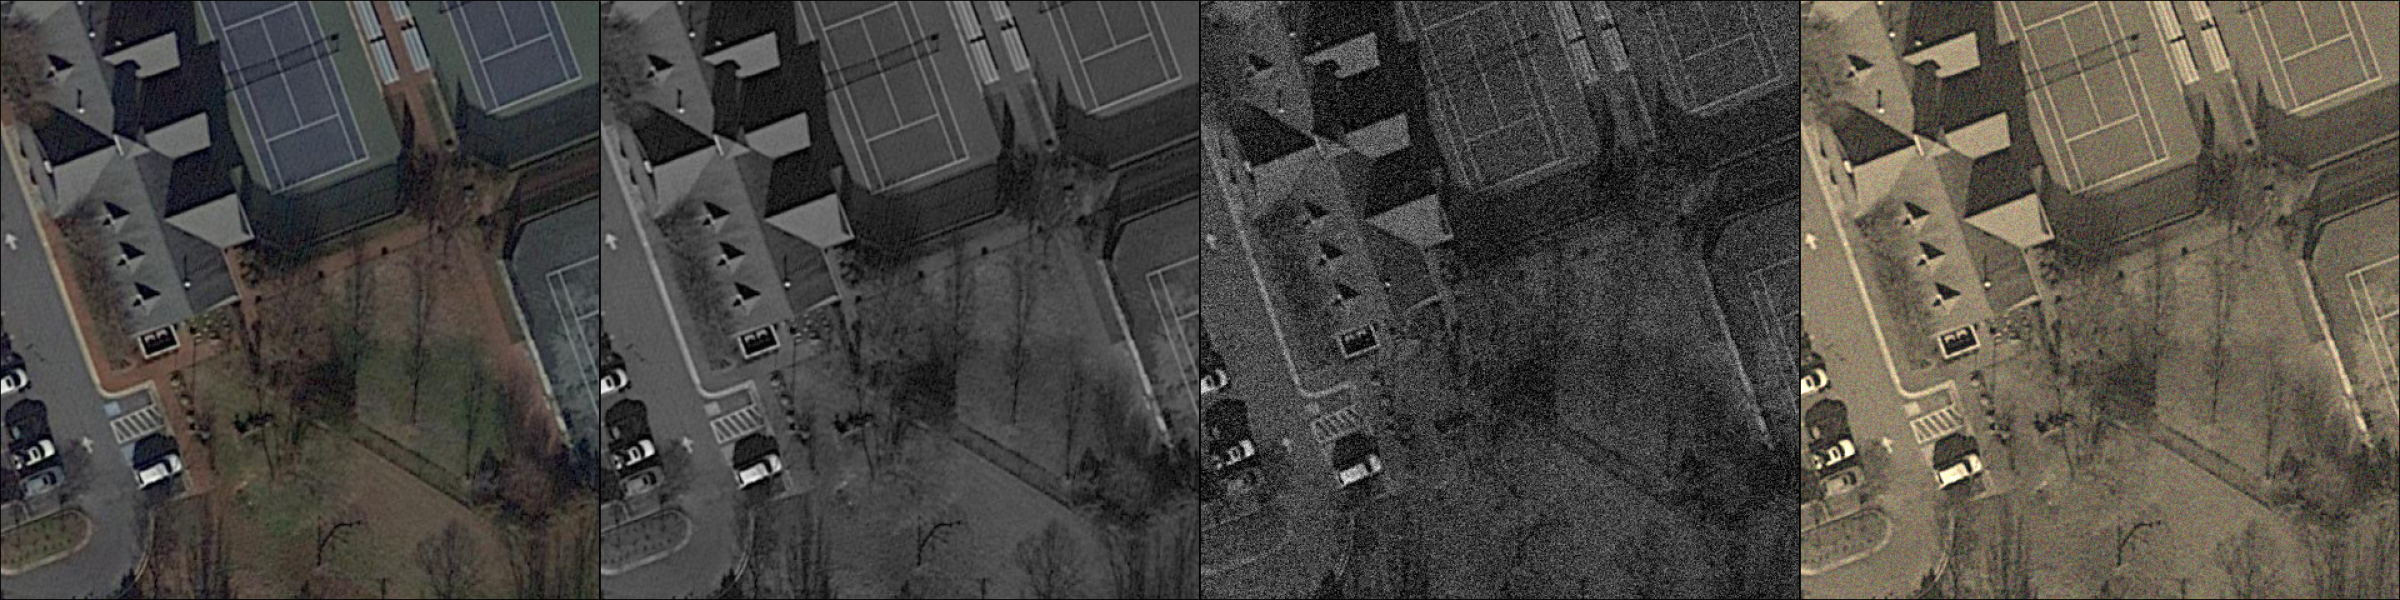
\includegraphics[width=0.9\textwidth]{./images/filters.png}
\caption{Comparison of original aerial image patch with three historic filter transformations: grayscale conversion, sepia toning, and Gaussian noise addition. These filters simulate common degradation patterns in historical aerial photography.}
\label{fig:historic_filters}
\end{figure*}

\subsection{Final Dataset Statistics}

The rule-based generation yields 506{,}194 starting expressions and identifies 259{,}709 annotated targets across the corpus (Table~\ref{tab:llm_enhancement_stats}). Building on this base, the LLM enhancement is prompted to produce one language variation for each original expression and two unique visual‑detail expressions for each target, adding 496{,}895 and 519{,}434 expressions respectively and resulting in 1{,}522{,}523 total expressions.


\begin{figure}[!t]
\centering
\includegraphics[width=\columnwidth]{./images/expression_wordcloud.png}
\caption{Word cloud visualization of the most frequent terms in Aerial-D referring expressions, highlighting the domain-specific vocabulary and spatial descriptors characteristic of aerial imagery.}
\label{fig:expression_wordcloud}
\end{figure}

\begin{figure*}[t]
\centering
\begin{minipage}{0.48\textwidth}
\centering
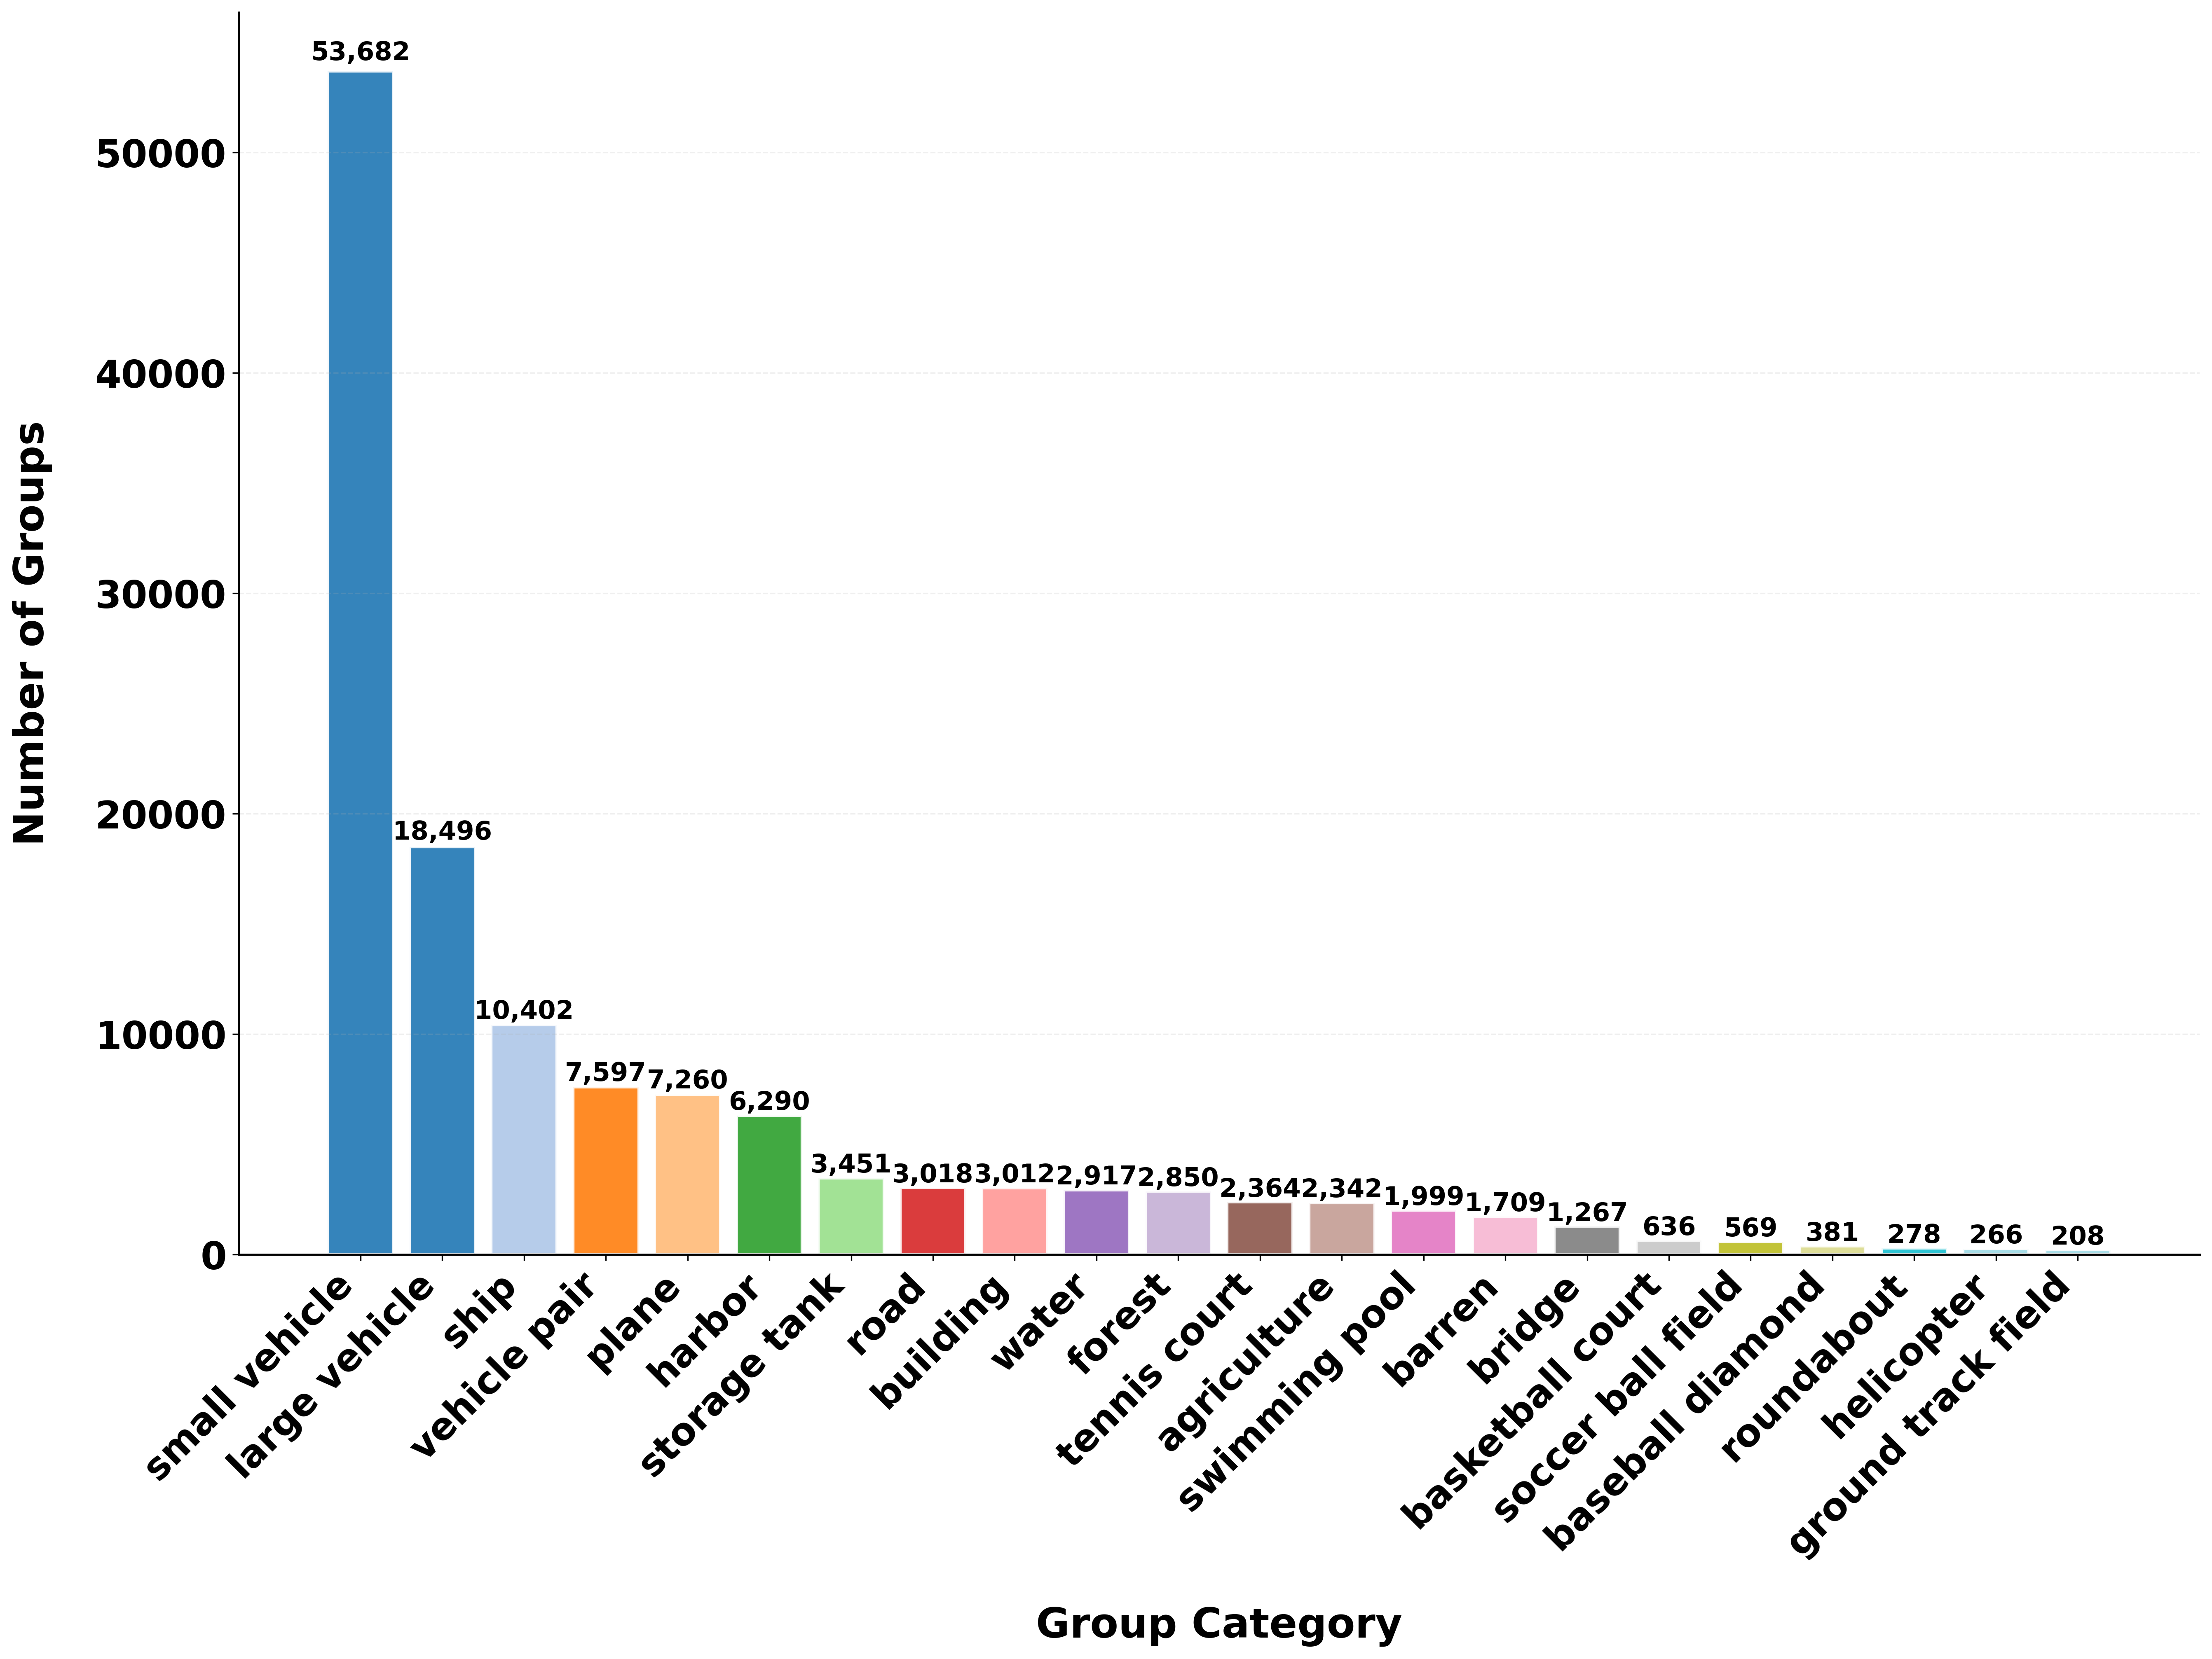
\includegraphics[width=\textwidth]{./images/group_category_distribution.png}
\end{minipage}\hfill
\begin{minipage}{0.48\textwidth}
\centering
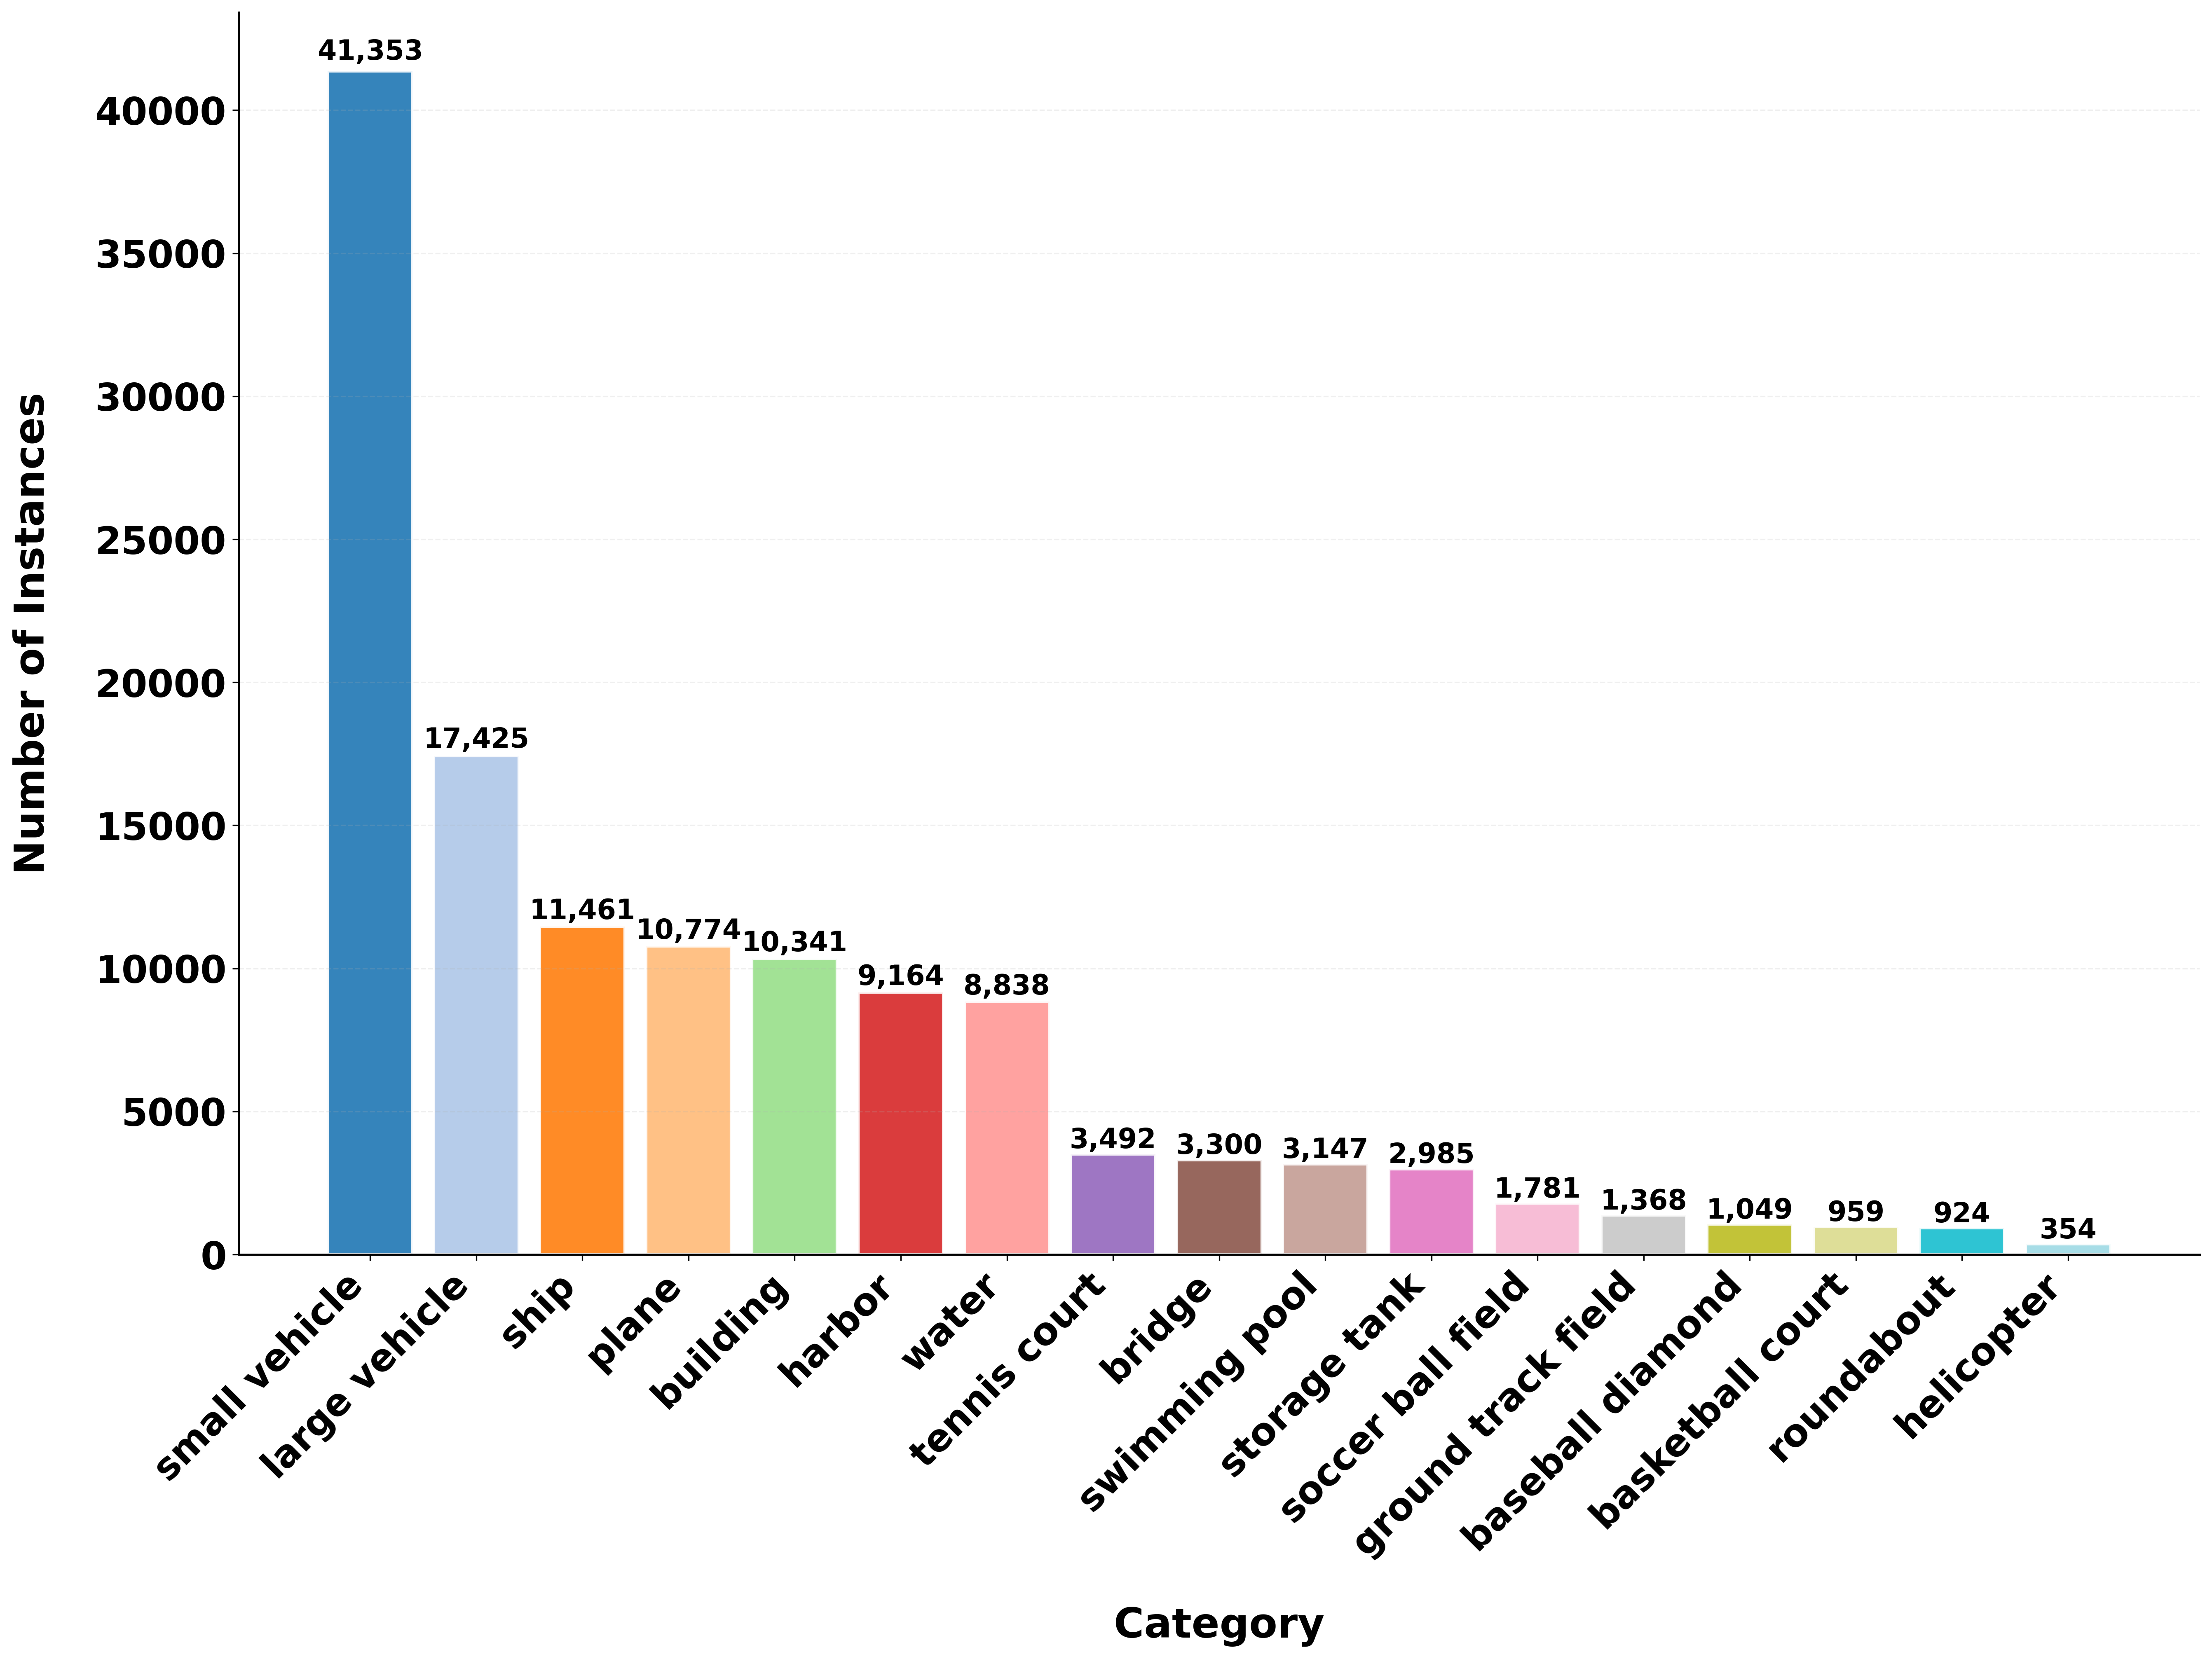
\includegraphics[width=\textwidth]{./images/instance_category_distribution.png}
\end{minipage}
\caption{Category distribution analysis of Aerial-D dataset. Left: Distribution of group annotations showing the prevalence of different object categories in group-level referring expressions. Right: Distribution of individual instance annotations across semantic categories, demonstrating the dataset's coverage of aerial object types.}
\label{fig:category_distributions}
\end{figure*}


Table \ref{tab:dataset_comparison} compares Aerial-D with prior RRSIS datasets and shows how it scales along three axes: images, targets per image, and expressions per target. First, Aerial-D contains nearly three times as many images as previous datasets. Second, each image typically includes many segmented targets. Third, each target is paired with multiple referring expressions. Together, these factors yield more than 1.5 million referring expressions, making Aerial-D the largest RRSIS resource to date. Beyond scale, Aerial-D is one of the first to use a fully automatic pipeline that combines rule-based generation with LLM enhancement and supports both single-object and multi-object references.

% Dataset comparison table
\begin{table*}[t]
\centering
\caption{Comparison with Existing RRSIS Datasets}
\label{tab:dataset_comparison}
\resizebox{\textwidth}{!}{%
\begin{tabular}{@{}lccccccr@{}}
\toprule
\textbf{Dataset} & \textbf{Image Resolution} & \textbf{Images} & \textbf{Annotations} & \textbf{Single-object} & \textbf{Multi-object} & \textbf{Resolution} & \textbf{Annotation Generation} \\
\midrule
RefSegRS & 0.13m & 4420 & 4420 & \checkmark & $\times$ & 512 & Manual \\
RRSIS-D & 0.5m-30m & 17402 & 17402 & \checkmark & $\times$ & 800 & Semi-auto \\
NWPU-Refer & 0.12m-0.5m & 15003 & 49745 & \checkmark & \checkmark & 1024-2048 & Manual \\
\midrule
\textbf{AERIAL-D} & \textbf{0.3m-4.5m} & \textbf{43,514} & \textbf{1,545,994} & \textbf{\checkmark} & \textbf{\checkmark} & \textbf{480} & \textbf{Automated + LLM} \\
\bottomrule
\end{tabular}%
}
\end{table*}

\begin{table}[H]
\centering
\caption{Expression Distribution by Source}
\label{tab:llm_enhancement_stats}
\footnotesize
\begin{tabular}{@{}lcc@{}}
\toprule
\textbf{Source} & \textbf{Train} & \textbf{Total} \\
\midrule
Rule-Based & 371K & 506K \\
LLM Language Variations & 364K & 497K \\
LLM Visual Details & 382K & 519K \\
\midrule
\textbf{Total} & \textbf{1,118K} & \textbf{1,523K} \\
\bottomrule
\end{tabular}
\end{table}

% Place the distillation pipeline figure near the end to avoid disrupting earlier figure order
\begin{figure}[!b]
\centering
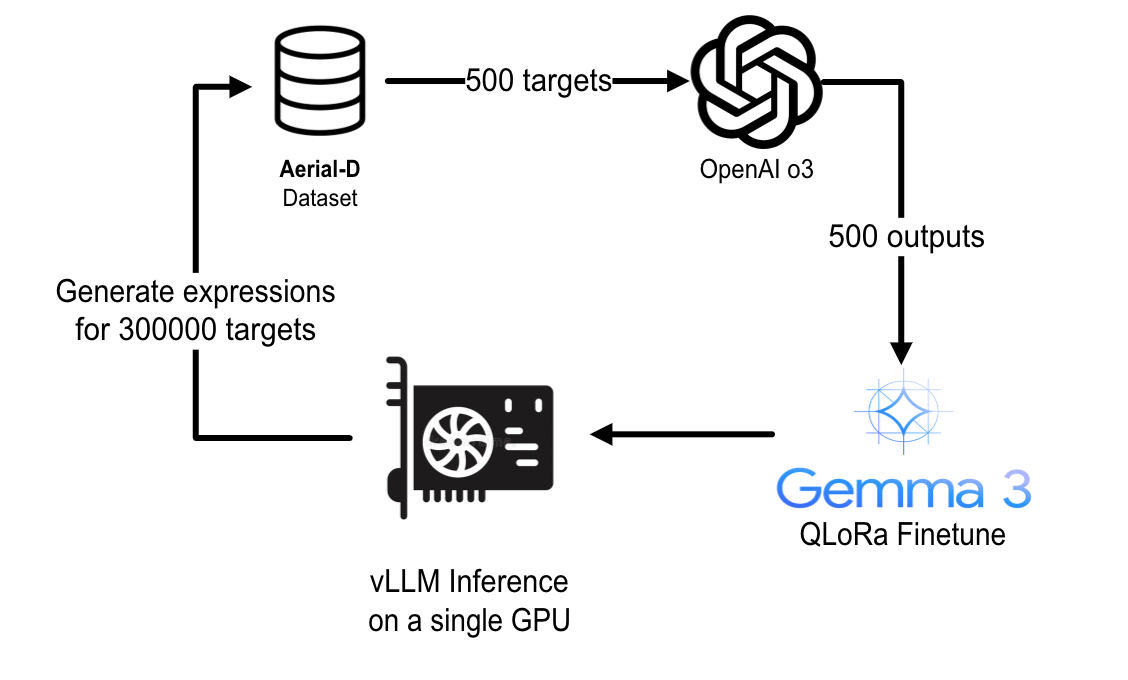
\includegraphics[width=\columnwidth]{./images/distillation.png}
\caption{Knowledge distillation pipeline for scalable LLM enhancement. A small sample of 500 expressions is processed through OpenAI's o3 model\cite{o3} to generate high-quality training targets, which are then used to fine-tune Gemma3‑12B\cite{gemma3} via QLoRA\cite{qlora}. The fine‑tuned model enables cost‑effective local inference to enhance the full dataset using vLLM\cite{vllm} on a single GPU.}
\label{fig:llm_distillation}
\end{figure}
